\documentclass[10pt]{article}

\usepackage[margin=1in]{geometry}
\usepackage[T1]{fontenc}
\usepackage[utf8]{inputenc}
\usepackage{lmodern}
\usepackage{microtype}
\usepackage{amsmath,amssymb}
\usepackage{booktabs}
\usepackage{xcolor}
\usepackage{enumitem}
\usepackage{hyperref}
\usepackage{placeins}
\usepackage{float}
\usepackage{needspace}
\usepackage{etoolbox}
\usepackage{tikz}
\usepackage{pgfplots}

\pgfplotsset{compat=1.18}
\usetikzlibrary{calc,positioning}
\raggedbottom
\widowpenalty=10000
\clubpenalty=10000
\displaywidowpenalty=10000
\pretocmd{\section}{\Needspace{10\baselineskip}}{}{}
\pretocmd{\subsection}{\Needspace{12\baselineskip}}{}{}
\BeforeBeginEnvironment{itemize}{\begin{samepage}\Needspace{7\baselineskip}}
\AfterEndEnvironment{itemize}{\end{samepage}}
\BeforeBeginEnvironment{enumerate}{\begin{samepage}\Needspace{7\baselineskip}}
\AfterEndEnvironment{enumerate}{\end{samepage}}

\hypersetup{
  colorlinks=true,
  linkcolor=blue!50!black,
  citecolor=blue!50!black,
  urlcolor=blue!50!black
}

\title{\textbf{Retention Before Retrieval:\\Why Graph-Aware Memory Eviction\\Matters for LLM Agents}}
\author{Minkyu Song \\ \small Department of Computer Science, Yonsei University \\ \small \texttt{smkgenesis@yonsei.ac.kr}}
\date{}

\begin{document}
\maketitle

\begin{abstract}
Budget-constrained LLM systems face two logically distinct memory problems: what to retrieve and what to retain. The retrieval problem has received extensive attention; the retention problem has not. We argue that retention is logically prior, because once a structurally necessary block has been evicted, no retrieval method can recover it from the active prompt-visible store.

We study that retention stage with \emph{Dependency-aware Semantic Garbage Collection} (DSGC), a minimal policy that augments query relevance with one-hop prerequisite propagation over a benchmark-supplied dependency graph. The goal is not to present a general agent-memory architecture, but to establish a clean base case for graph-aware retention. The experimental package is fully fixed and public: after an initial preregistered run and documented postmortem, we redesign the benchmark, calibrate template families, freeze a paper-facing main suite, and then run a final robustness pack. In the main suite, all methods solve the control templates perfectly, while DSGC shows large gains on structurally indirect targets, where the needed prerequisite block is not itself strongly similar to the query. Under the lexical feature-hashing encoder, target full-chain retention is 0.90 for DSGC versus 0.03 for retrieval-only and no-graph baselines. Under the sentence encoder, the gap is 1.00 versus 0.23. Robustness experiments show that the gain persists across a moderate $\lambda_\pi$ range, appears most clearly at intermediate budgets, and weakens at larger scale for lexical targets. The resulting claim is that one-hop dependency propagation is sufficient to change retention behavior in a benchmarked indirect-prerequisite regime. This paper therefore proposes a framing as well as a result: retention before retrieval should be treated as a first-class memory problem.
\end{abstract}

\section{Introduction}

Long-horizon LLM systems routinely compress context because prompt space is limited. Common baselines retain recent tokens, retrieve past text by similarity, or page memories in and out heuristically. These strategies often work well when the needed evidence is either recent or lexically similar to the current query. They are less reliable when success depends on an \emph{older prerequisite} that remains structurally necessary while becoming semantically indirect with respect to the final query.

We refer to such a block as a \emph{structurally indirect prerequisite}: a block whose text is not itself strongly aligned with the query, but whose retention is necessary for recovering the correct answer.

This paper studies that specific failure mode. The central premise is that memory quality is not only a retrieval problem; it is also a retention problem. Most existing approaches effectively frame memory as a retrieval problem: given a query, search a store that is assumed to still contain the needed evidence. Budget-constrained LLM systems face an earlier failure point. Evidence can be permanently discarded before the query arrives, and once an upstream prerequisite has been evicted, no retrieval method can recover it from the active prompt-visible store. Retention is therefore logically prior to retrieval in the failure chain: if retention fails, retrieval operates on an incomplete memory state. We study that retention stage directly rather than proposing another retrieval variant.

We therefore study a minimal dependency-aware policy, DSGC, that adds a one-hop propagation term to similarity-based retention. The policy uses no learned controller, no multi-hop diffusion, and no hidden graph recall. The question is whether the smallest nontrivial graph-aware retention rule already changes behavior. In that sense, the paper is best understood as a base-case study for graph-based memory management under a broader framing: \emph{retention before retrieval}.

The paper makes four concrete contributions.
\begin{enumerate}[leftmargin=1.3em]
  \item It formulates an empirical claim around \emph{structurally indirect prerequisites}, positioning DSGC as a base case for graph-aware retention.
  \item It designs a benchmark and two-stage calibration-then-freeze protocol that cleanly separates retrieval-friendly controls from dependency-sensitive targets.
  \item It shows that in the frozen main suite, retrieval-only and no-graph DSGC coincide, while one-hop DSGC yields large target gains with no control advantage.
  \item It documents robustness and limitations explicitly, including budget curves, $\lambda_\pi$ sensitivity, a sliding-window baseline, and mixed scale behavior at larger block counts.
\end{enumerate}

\section{Retrieval vs.\ Retention}

\subsection{The Retrieval Paradigm}

Our setting is adjacent to retrieval-augmented language modeling and question answering, including RAG, REALM, RETRO, and Atlas \cite{rag2020,realm2020,retro2021,atlas2022}. These systems focus on augmenting generation with external retrieval, typically to improve factual access over large corpora. They answer the question ``how should a model fetch supporting evidence?'' Crucially, they assume that the relevant evidence is still present in the store at query time. Our question is earlier in the pipeline: under a fixed prompt budget, what should remain in memory before retrieval is even attempted? If a structurally necessary block has already been evicted, better retrieval cannot recover it from the active store.

The paper is also related to graph-augmented retrieval and knowledge access, including GraphRAG and HippoRAG \cite{graphrag2024,hipporag2024}. Those methods use graph structure to expand, organize, or rank retrieved evidence over a store that is again assumed to be complete. DSGC studies a qualitatively earlier use of graph structure: not how to traverse a store more effectively, but how to decide which nodes to keep before budget pressure makes later retrieval impossible. It therefore asks whether the minimal graph-aware retention rule, namely one-hop prerequisite propagation, already changes prompt-visible memory behavior.

\subsection{The Retention Gap}

Agent-memory systems and long-horizon agent architectures provide a second point of contact. MemGPT, SCM, Generative Agents, Reflexion, Voyager, and LATS all show that external memory, reflection, and planning are central to extended agent behavior \cite{memgpt2023,scm2023,generative_agents2023,reflexion2023,voyager2023,lats2024}. However, these systems do not isolate the specific mechanism studied here: preserving an upstream prerequisite whose text is weakly aligned with the final query. They demonstrate that memory management matters, but they do not separate the retention decision from the broader agent loop. Our contribution is therefore not a broader agent architecture, but a controlled base-case study of the retention decision itself, isolated from the rest of the agent loop.

Finally, the work touches context compression and prompt reduction methods such as Gisting and LongLLMLingua \cite{gisting2023,longllmlingua2023}. Those methods ask how to fit more information into a bounded context by compressing or summarizing prompts. They change the representation of what is kept, but they do not directly study which blocks should survive an eviction decision under structural dependence. At a conceptual level, the work is also related to curriculum-style prerequisite structure and staged task decomposition \cite{curriculum2009}. DSGC addresses that dependence not through training order, but through prompt-level eviction decisions at inference time.

\subsection{This Work: Retention as a First-Class Problem}

The central claim of this paper is not that retrieval is unimportant, but that it is incomplete as a framing for memory management under budget pressure. Retention and retrieval are distinct stages with different failure modes. Existing work has concentrated overwhelmingly on retrieval over stores that still contain the needed evidence. This paper argues that retention deserves independent study because store incompleteness can arise \emph{before} retrieval is ever invoked. DSGC is therefore presented as a first instance within a broader retention-before-retrieval framework rather than as a complete memory architecture.

\section{Method}

\paragraph{Problem statement.}
Given a memory store of $N$ blocks, a query, and a token budget $B < \sum_i s_i$, select a subset of blocks whose total cost does not exceed $B$. The goal is to maximize the probability that all structurally necessary blocks are retained in the prompt-visible store. This is a retention problem, not a retrieval problem: once a block has been discarded under the budget, it cannot be retrieved later from the active memory state.

\subsection{Blocks and Graph}

At a query step, the memory store contains blocks $\mathcal{B} = \{b_1,\dots,b_N\}$. Each block has text, a token cost, and an optional set of prerequisite edges supplied by the benchmark. An edge $(j,i)$ means that block $j$ depends on block $i$, so $i$ is a prerequisite of $j$.

The benchmark provides the graph. This isolates the retention question from graph induction. We do not claim that real agent traces already come with clean prerequisite edges; we ask what graph-aware memory management can already achieve once such structure is available.

\subsection{Encoders}

We evaluate two encoders already implemented in the public codebase. The first is a deterministic 256-dimensional feature-hashing encoder over alphanumeric tokens. It is simple and stable for local reproduction, and it serves as a lexical baseline whose behavior is easy to audit. The second is a sentence encoder backed by \texttt{sentence-transformers} using \texttt{all-MiniLM-L6-v2}, producing 384-dimensional normalized embeddings. The paper uses both because some failures are mostly lexical, while others remain structural even under a stronger semantic encoder.

\subsection{Scoring Rule}

For query embedding $\mathbf{g}$ and block embedding $\mathbf{e}_i$, we compute raw relevance scores with a dot product and normalize them with a softmax:
\[
r_i = \mathrm{softmax}\!\left(\frac{\mathbf{g}^\top \mathbf{e}_i}{\tau}\right).
\]
In all paper-facing experiments, the relevance temperature is fixed at $\tau=0.25$.

The only graph term used in the paper-facing policy is one-hop prerequisite propagation:
\[
\pi_i = \sum_{j : (j,i)\in E} r_j.
\]
The DSGC score is then
\[
I_i = r_i + \lambda_\pi \pi_i.
\]
Intuitively, if a downstream block $j$ is highly relevant to the current query, its prerequisite $i$ inherits part of that relevance through $\pi_i$. This is precisely the intended rescue mechanism: a structurally necessary block should not be discarded merely because its own text is only weakly aligned with the query.

In the main suite, $\lambda_\pi = 1.0$. The no-graph ablation uses the same implementation with graph propagation disabled, so the comparison is \emph{within the same code path}. This was an explicit design requirement after the earlier repository iterations, because a base-case claim is only credible if the graph term is isolated cleanly.

\subsection{Budgeted Selection}

In all experiments, the density exponent is fixed at $\alpha = 0$, so blocks are selected greedily in descending order of $I_i$ until the L1 budget is exhausted. The only policy difference between DSGC and the no-graph ablation is the one-hop propagation term.

This base-case formulation also keeps the cost structure simple. If there are $N$ candidate blocks with embedding dimension $d$, relevance scoring is a matrix-vector style operation with cost $O(Nd)$. One-hop propagation adds a sparse graph pass with cost $O(E)$ over dependency edges, and final selection adds $O(N \log N)$ under full sorting or a standard top-$k$ routine of comparable practical cost. The complete score-to-selection cycle is therefore transparent: $O(Nd + E + N \log N)$. The paper thus studies the smallest graph-aware intervention that is both empirically identifiable and computationally lightweight.

\begin{figure}[t]
\centering
\resizebox{0.88\linewidth}{!}{%
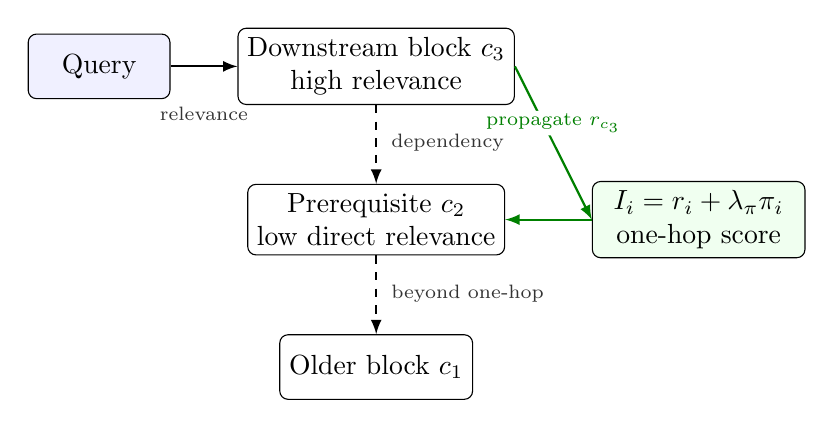
\begin{tikzpicture}[
  block/.style={draw, rounded corners=3pt, minimum width=2.3cm, minimum height=0.82cm, align=center, line width=0.4pt},
  query/.style={draw, rounded corners=3pt, fill=blue!6, minimum width=1.8cm, minimum height=0.82cm, align=center, line width=0.4pt},
  note/.style={draw, rounded corners=3pt, fill=green!6, minimum width=2.7cm, minimum height=0.82cm, align=center, line width=0.4pt},
  ann/.style={inner sep=1pt, font=\scriptsize, text=black!80},
  propann/.style={fill=white, inner sep=1pt, rounded corners=2pt, font=\scriptsize, text=green!50!black},
  arr/.style={-latex, thick},
  dep/.style={-latex, thick, dashed}
]
\node[query] (query) {Query};
\node[block, right=0.85cm of query] (c3) {Downstream block $c_3$\\high relevance};
\node[block, below=1.0cm of c3] (c2) {Prerequisite $c_2$\\low direct relevance};
\node[block, below=1.0cm of c2] (c1) {Older block $c_1$};
\node[note, right=1.1cm of c2] (score) {$I_i = r_i + \lambda_\pi \pi_i$\\one-hop score};

\draw[arr] (query) -- (c3);
\draw[dep] (c3) -- (c2);
\draw[dep] (c2) -- (c1);
\draw[arr, green!50!black] (c3.east) -- (score.west);
\draw[arr, green!50!black] (score.west) -- ++(-0.55,0) |- (c2.east);
\node[ann] at ($(query.east)!0.5!(c3.west)+(0,-0.6)$) {relevance};
\node[ann, anchor=west] at ($(c3)!0.5!(c2)+(0.15,0)$) {dependency};
\node[ann, anchor=west] at ($(c2)!0.5!(c1)+(0.15,0)$) {beyond one-hop};
\node[propann] at ($(c3)!0.55!(score)+(0,0.35)$) {propagate $r_{c_3}$};
\end{tikzpicture}
}
\caption{DSGC mechanism. A query-relevant downstream block can rescue its immediate prerequisite through one-hop propagation; the policy does not extend to multi-hop propagation.}
\label{fig:system}
\end{figure}

\section{Benchmark and Protocol}

\subsection{Template Families}

The benchmark contains control and target families.

\textbf{Controls.} \texttt{budget\_control} and \texttt{numeric\_threshold\_control\_v2} are retrieval-friendly. They are designed so that the final query directly overlaps with the chain blocks it needs, making graph propagation unnecessary in the clean case. In \texttt{budget\_control}, one block gives a project budget and another gives the approval margin relative to that budget; the final query simply asks whether a proposed cost is allowed. Because the project name, budget quantity, and approval language all reappear in the query, similarity-only retrieval is already enough. \texttt{numeric\_threshold\_control\_v2} plays the same role with threshold-style wording: the decisive numeric rule is itself query-facing, so the benchmark behaves like a standard retrieval problem rather than a dependency-sensitive one. In the redesign phase, a third candidate control (\texttt{permission\_control\_v2}) was rejected because retrieval-only solved it too inconsistently to qualify as a clean control. We keep that rejection in the repository history rather than silently removing it.

\textbf{Targets.} \texttt{opaque\_role\_target\_v2} and \texttt{opaque\_profile\_target\_v2} are structurally indirect. They require keeping an upstream block whose role is necessary for the answer but not directly favored by similarity alone. In \texttt{opaque\_role\_target\_v2}, the query asks whether a user may delete the backup, so the downstream decision block is query-relevant, the middle mapping block is rescued by one hop, and the oldest assignment block still survives by shared keywords. This makes it the cleanest target: the graph term matters, but the oldest block still gets some lexical help. In \texttt{opaque\_profile\_target\_v2}, by contrast, the query is about direct partner routing while the oldest block only links the service to an intermediate ticket, so that earliest prerequisite receives much weaker direct support and is the first block likely to be displaced under budget pressure. This is why the profile template is the hardest target in the suite and the best place to observe residual one-hop failure. Figure~\ref{fig:target-contrast} illustrates this contrast directly. The final v2 templates were renamed and rebuilt after a postmortem on earlier encoder-sensitive artifacts.

\begin{figure}[t]
\centering
\resizebox{0.95\linewidth}{!}{%
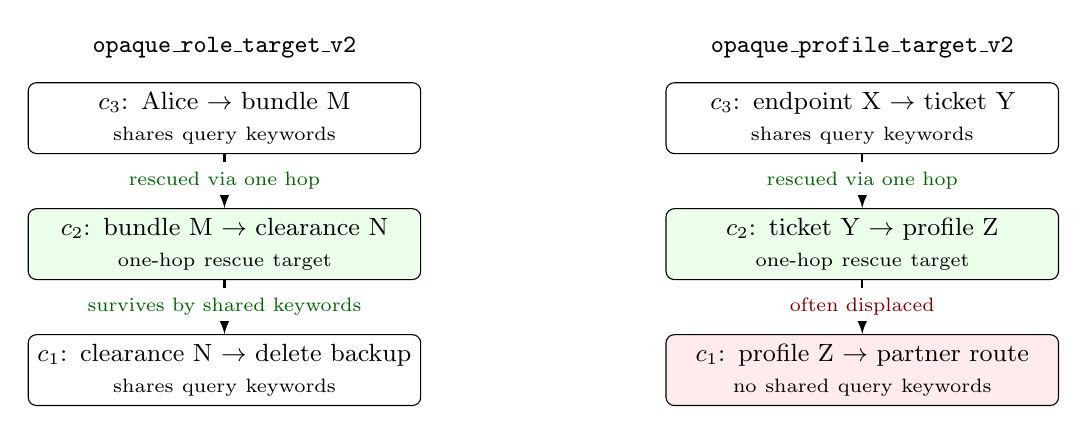
\begin{tikzpicture}[
  box/.style={draw, rounded corners=3pt, text width=4.75cm, minimum height=0.9cm, align=center, line width=0.4pt, font=\small},
  qbox/.style={box, fill=green!8},
  nbox/.style={box, fill=white},
  wbox/.style={box, fill=red!8},
  midlbl/.style={font=\scriptsize, text=green!40!black, fill=white, inner sep=2pt},
  midlblf/.style={font=\scriptsize, text=red!50!black, fill=white, inner sep=2pt},
  dep/.style={-latex, thick, dashed},
]
% === Left panel ===
\node[font=\small\bfseries] at (-0.3,3.6) {\texttt{opaque\_role\_target\_v2}};
\node[nbox] (Lc3) at (-0.3,2.7) {$c_3$: Alice $\to$ bundle M\\{\scriptsize shares query keywords}};
\node[qbox] (Lc2) at (-0.3,1.1) {$c_2$: bundle M $\to$ clearance N\\{\scriptsize one-hop rescue target}};
\node[nbox] (Lc1) at (-0.3,-0.5) {$c_1$: clearance N $\to$ delete backup\\{\scriptsize shares query keywords}};
\draw[dep] (Lc3) -- (Lc2);
\draw[dep] (Lc2) -- (Lc1);
\node[midlbl] at (-0.3,1.9) {rescued via one hop};
\node[midlbl] at (-0.3,0.3) {survives by shared keywords};
% === Right panel ===
\node[font=\small\bfseries] at (7.8,3.6) {\texttt{opaque\_profile\_target\_v2}};
\node[nbox] (Rc3) at (7.8,2.7) {$c_3$: endpoint X $\to$ ticket Y\\{\scriptsize shares query keywords}};
\node[qbox] (Rc2) at (7.8,1.1) {$c_2$: ticket Y $\to$ profile Z\\{\scriptsize one-hop rescue target}};
\node[wbox] (Rc1) at (7.8,-0.5) {$c_1$: profile Z $\to$ partner route\\{\scriptsize no shared query keywords}};
\draw[dep] (Rc3) -- (Rc2);
\draw[dep] (Rc2) -- (Rc1);
\node[midlbl] at (7.8,1.9) {rescued via one hop};
\node[midlblf] at (7.8,0.3) {often displaced};
\end{tikzpicture}%
}
\caption{Why the two target templates differ. In \texttt{opaque\_role\_target\_v2}, the query about whether a user may delete the backup keeps the downstream decision block relevant, rescues the middle mapping block through one-hop propagation, and still gives the oldest assignment block enough lexical support to survive. In \texttt{opaque\_profile\_target\_v2}, the query about direct partner routing again rescues the middle block, but the oldest service-to-ticket block receives little direct support and is therefore the first block to drop.}
\label{fig:target-contrast}
\end{figure}

Each scenario also contains \emph{honeypots}: distractor blocks designed to share some query vocabulary without completing the correct reasoning chain. They are necessary because, without such distractors, the benchmark would collapse into trivial recency or lexical retrieval. The calibration stage varied honeypot count and strength, and the frozen main suite uses the medium-strength setting selected from that calibration.

The resulting four-template suite is intentionally small. The controls establish that the benchmark can behave like ordinary similarity-based retrieval when the decisive rule is query-facing. The targets then isolate the opposite regime: the answer still depends on a short chain, but one prerequisite becomes structurally necessary before it becomes lexically attractive. This control-target symmetry matters more for the paper than raw template count. The point is not to enumerate many superficially different tasks, but to pin down a narrow causal contrast in which one-hop graph bias should matter only in the indirect cases and should disappear in the direct ones.

\subsection{Experimental History}

The public codebase preserves the experiment history instead of exposing only the winning run.
\begin{enumerate}[leftmargin=1.3em]
  \item \texttt{final\_v1}: initial preregistered four-experiment suite.
  \item \texttt{final\_v1} postmortem: documented failure analysis and redesign rationale.
  \item \texttt{final\_v2} calibration: used to select clean controls, target families, and operating regimes.
  \item \texttt{final\_v2\_main}: frozen paper-facing main suite.
  \item \texttt{final\_v3\_robustness}: final sensitivity and limitation pack.
\end{enumerate}
This sequence matters because the paper is not claiming that the first benchmark draft was already correct. The redesign history is part of the scientific record, not an inconvenience to be hidden.

\Needspace{18\baselineskip}
\subsection{Frozen Main Suite}

The fixed \texttt{final\_v2\_main} protocol uses:
\begin{itemize}[leftmargin=1.3em]
  \item 4 templates: 2 controls and 2 targets;
  \item methods: retrieval-only, no-graph DSGC, and DSGC;
  \item encoders: frozen and sentence;
  \item 15 seeds;
  \item total block count 20;
  \item medium-strength honeypots;
  \item control settings: chain depth 2, 4 honeypots, budget multiplier 2.0;
  \item target settings: chain depth 3, 2 honeypots, budget multiplier 2.0.
\end{itemize}

The primary metric is \texttt{full\_chain\_retention}. We also track prerequisite retention and answer accuracy, but in the final suite answer accuracy is effectively redundant with full-chain retention and is treated as secondary.

The preregistered predictions were:
\begin{enumerate}[leftmargin=1.3em]
  \item controls: retrieval-only should achieve at least 0.90 and DSGC should match it;
  \item targets: DSGC should outperform both retrieval-only and no-graph DSGC;
  \item \texttt{opaque\_role\_target\_v2} should remain the cleanest target;
  \item \texttt{opaque\_profile\_target\_v2} should preserve a positive DSGC advantage under the sentence encoder.
\end{enumerate}

\section{Main Results}

Table~\ref{tab:main-regime} shows the paper-facing regime averages. The control story is completely clean: all three methods achieve perfect full-chain retention under both encoders. The target story is equally clear: retrieval-only and no-graph DSGC coincide, while DSGC is much stronger.

\begin{table}[H]
\centering
\small
\begin{tabular}{llll}
\toprule
Encoder & Regime & Method & Full-chain retention \\
\midrule
Frozen & Control & Retrieval-only & 1.0000 $\pm$ 0.0000 \\
Frozen & Control & No-graph DSGC & 1.0000 $\pm$ 0.0000 \\
Frozen & Control & DSGC & 1.0000 $\pm$ 0.0000 \\
Frozen & Target & Retrieval-only & 0.0333 $\pm$ 0.1826 \\
Frozen & Target & No-graph DSGC & 0.0333 $\pm$ 0.1826 \\
Frozen & Target & DSGC & 0.9000 $\pm$ 0.3051 \\
Sentence & Control & Retrieval-only & 1.0000 $\pm$ 0.0000 \\
Sentence & Control & No-graph DSGC & 1.0000 $\pm$ 0.0000 \\
Sentence & Control & DSGC & 1.0000 $\pm$ 0.0000 \\
Sentence & Target & Retrieval-only & 0.2333 $\pm$ 0.4302 \\
Sentence & Target & No-graph DSGC & 0.2333 $\pm$ 0.4302 \\
Sentence & Target & DSGC & 1.0000 $\pm$ 0.0000 \\
\bottomrule
\end{tabular}
\caption{Regime-level full-chain retention in the fixed \texttt{final\_v2\_main} suite.}
\label{tab:main-regime}
\end{table}

The template-level picture is consistent with the preregistration and also shows that the profile target is harder than the role target.

\begin{table}[H]
\centering
\small
\begin{tabular}{lllll}
\toprule
Encoder & Target template & Retrieval-only & No-graph DSGC & DSGC \\
\midrule
Frozen & \texttt{opaque\_role\_target\_v2} & 0.0000 $\pm$ 0.0000 & 0.0000 $\pm$ 0.0000 & 1.0000 $\pm$ 0.0000 \\
Frozen & \texttt{opaque\_profile\_target\_v2} & 0.0667 $\pm$ 0.2582 & 0.0667 $\pm$ 0.2582 & 0.8000 $\pm$ 0.4140 \\
Sentence & \texttt{opaque\_role\_target\_v2} & 0.1333 $\pm$ 0.3519 & 0.1333 $\pm$ 0.3519 & 1.0000 $\pm$ 0.0000 \\
Sentence & \texttt{opaque\_profile\_target\_v2} & 0.3333 $\pm$ 0.4880 & 0.3333 $\pm$ 0.4880 & 1.0000 $\pm$ 0.0000 \\
\bottomrule
\end{tabular}
\caption{Target-template full-chain retention in the main suite (mean $\pm$ standard deviation over 15 seeds).}
\label{tab:target-templates}
\end{table}

Two aspects of Table~\ref{tab:main-regime} matter most.

First, the control result rules out the trivial interpretation that DSGC simply adds a blanket advantage everywhere. It does not. In retrieval-friendly settings, DSGC has no measurable edge because there is no structural dependency for the graph term to rescue.

Second, the near-exact equality between retrieval-only and no-graph DSGC is important. This equality is not accidental. With graph propagation disabled, the policy score reduces to $I_i=r_i$, and $r_i$ is just a softmax over raw dot-product scores. Since softmax preserves ranking, no-graph DSGC and retrieval-only induce the same block ordering. The gain is therefore not coming from an unrelated implementation difference; it is tied to the one-hop propagation term itself, which is exactly what a base-case graph-memory argument requires.

\FloatBarrier

\section{Robustness and Limitations}

\subsection{Sensitivity and Budget Curves}

The \texttt{final\_v3\_robustness} pack adds four checks: a $\lambda_\pi$ sweep, a budget curve, a sliding-window baseline, and a scale test.

Across $\lambda_\pi \in \{0.5,1.0,2.0\}$, target gains remain positive. On frozen \texttt{opaque\_profile\_target\_v2}, DSGC moves from 0.6667 to 0.8000 to 0.8667 as $\lambda_\pi$ increases, while retrieval-only remains at 0.0667. On frozen \texttt{opaque\_role\_target\_v2}, DSGC remains at 1.0000 across all three values while retrieval-only stays at 0.0000.

The budget curve reveals the intended operating-range story. At tight budgets, all methods may fail because there is simply not enough room for the chain. At intermediate budgets, DSGC separates sharply from retrieval-only. At loose budgets, retrieval-only and no-graph DSGC begin to catch up. For instance, on frozen \texttt{opaque\_profile\_target\_v2}, DSGC improves from 0.5333 at multiplier 1.0 to 0.8000 at 2.0 and 1.0000 at 5.0, whereas retrieval-only moves from 0.0000 to 0.0667 to 0.6000 over the same budgets. The retrieval-only curve is not perfectly monotone: at multiplier 5.0 on frozen \texttt{opaque\_role\_target\_v2}, the larger budget admits additional filler and honeypot blocks whose frozen-encoder scores remain competitive with the chain, so a chain block can still be displaced even after a smaller budget happened to retain it. This is the narrow operating-range claim of the paper: dependency-aware retention matters most before the budget becomes loose enough to keep nearly everything anyway.

\subsection{Sliding Window Baseline}

The sliding-window baseline remains weak throughout the budget sweep. At budget multiplier 2.0, it reaches only 0.0667 on all four frozen templates, including the controls. This is not the primary scientific comparison, but it answers the obvious reviewer question about a naive recency baseline. The failure is expected: in these tasks, recency is neither equivalent to relevance nor sufficient to preserve the prerequisite chain. We do not include a random selector because it would be strictly weaker than both recency and similarity baselines and therefore adds little diagnostic value beyond those stronger comparators.

\subsection{Scale}

The strongest limitation is scale. Controls remain perfect at 50 total blocks, and sentence-encoder DSGC stays strong on the targets. The frozen-encoder targets do not. In the frozen setting, the profile target drops from 0.8000 at 20 blocks to 0.3333 at 50 blocks, and the role target drops from 1.0000 to 0.7333. A plausible mechanism is that, as the candidate pool grows, relevance mass spreads across more distractors and the one-hop propagation signal has to compete with a larger set of semantically similar blocks. We therefore do \emph{not} claim that the current method is scale-robust in general.

\subsection{Failure Diagnosis}

The codebase records rank and displacement diagnostics for each run. In the three frozen profile-target failures of the main suite, the immediate issue is displacement of the oldest prerequisite block \texttt{c1}. In those failed seeds, \texttt{c2} and \texttt{c3} rank first and second, while \texttt{c1} falls to rank 10, 6, and 6 respectively and is displaced by non-chain blocks. This matters because it grounds the remaining failure in public diagnostics rather than in post hoc speculation.

\section{Discussion}

The paper supports the following empirical statement:
Under fixed prompt budgets, one-hop dependency propagation is sufficient to improve retention when the answer depends on structurally necessary but semantically indirect prerequisites.

This positions the contribution at the retention stage of memory management, which is logically prior to retrieval. Much of the existing literature has focused on retrieval: how to find relevant evidence in a store that still contains it. The present results suggest that retention deserves independent study, because structural prerequisites can be lost before retrieval is ever invoked.

This is not a claim that ``graph memory beats retrieval'' or that ``DSGC solves long-horizon memory.'' What the paper establishes is a constructive first case: once structural dependence is made explicit, even one-hop graph bias changes retention behavior in a way that similarity-only policies do not match. Several scope boundaries apply.

\begin{itemize}[leftmargin=1.3em]
  \item The benchmark uses supplied dependency graphs rather than inferred ones.
  \item The strongest evidence comes from synthetic template families chosen after an explicit redesign process.
  \item Robustness at larger block counts is mixed, especially for the frozen encoder.
  \item The answer metric is not independent of full-chain retention in the final suite.
\end{itemize}

At the same time, the evidence is stronger than a single benchmark win. The repository includes a failed first version, a postmortem, a calibration run, a frozen main suite, and a separate robustness pack. That visible iteration history is part of why the claim is credible.

The largest practical limitation is that the experiments assume supplied dependency graphs. Future work could therefore explore lightweight graph induction over agent traces, multi-hop propagation, and incremental graph-aware memory stores. More broadly, the retention-before-retrieval framing suggests inferring dependency edges from traces, testing whether multi-hop propagation helps at larger scale, co-optimizing retention and retrieval, and adapting policies to changing budgets. The broader implication is not that graph memory is solved, but that even minimal structural awareness is already strong enough to justify pursuing those richer directions.

\subsection{Hardware and Systems Considerations}

The one-hop restriction is not only a conceptual choice; it also preserves a favorable systems profile. The relevance term $r_i$ is a dense query--block inner product, the propagation term $\pi_i$ is a single sparse pass implementable as SpMV or scatter-add, and final retention reduces to score ordering plus a standard top-$k$ budgeted selection step. The resulting cost is $O(Nd + E + N \log N)$, where $N$ is the number of candidate blocks, $d$ is embedding dimension, and $E$ is the number of dependency edges. When the graph is sparse, the extra structural cost follows declared prerequisite edges rather than an $O(N^2)$ all-pairs interaction pattern. That does not make DSGC universally cheaper than every alternative, but it does make the base case algorithmically lightweight enough to be plausible as an online memory-management component.

Moving beyond one hop would preserve those sparse primitives but lose the single-pass property. A $k$-hop DSGC would look more like iterative SpMV or repeated scatter-add, pushing propagation toward $O(kE)$, increasing synchronization overheads, and introducing possible score amplification or diffusion artifacts that may require damping or normalization. We therefore treat multi-hop DSGC not as a free extension, but as a separate systems problem with new efficiency and stability tradeoffs.

We do \emph{not} benchmark kernel-level latency, throughput, or memory overhead on a production inference stack. The claim is narrower: the base-case rule is substantially simpler than full graph neural reasoning and structurally more hardware-friendly than repeated global recomputation.

The same separation matters for graph induction. In realistic deployments, edge construction need not sit on the per-step retention hot path; if edges are created when blocks are ingested or updated, the induction cost is amortized over later retention cycles. In trace-rich agents, some dependencies may also be recoverable from execution logs, tool-call traces, or other lightweight monitors rather than from repeated LLM inference. We do not benchmark that path here, but it suggests a plausible deployment route in which graph maintenance remains materially cheaper than repeating a more expensive memory-reasoning procedure at every step.

\section{Reproducibility and Open-Source Artifact}

The curated public release is published at \url{https://github.com/smkgenesis/dsgc}; running \path{reproduce.sh} recreates the paper-facing \texttt{final\_v2\_main} and \texttt{final\_v3\_robustness} outputs and preserves the redesign history.

\section{Conclusion}

This paper defines a benchmarked indirect-prerequisite failure mode, evaluates a one-hop graph-aware retention rule against matched baselines, and releases the resulting protocol as a public artifact. The main suite cleanly separates retrieval-friendly controls from dependency-sensitive targets, while the robustness pack shows that the effect survives moderate hyperparameter variation and is concentrated in the intermediate-budget regime. The result does not establish general graph-based memory management, but it does establish a transparent empirical base case for graph-aware retention as the logically prior stage in the retention-before-retrieval framing.

\begingroup
\small
\bibliographystyle{plain}
\bibliography{references}
\endgroup

\appendix
\small

\section{Target Lambda Sweep}

Table~\ref{tab:appendix-lambda} gives the target-only $\lambda_\pi$ sweep. The
role target is saturated throughout, while the frozen profile target improves
gradually as propagation weight increases.

\begin{table}[h]
  \centering
  \footnotesize
\begin{tabular}{lllll}
\toprule
Template & Encoder & $\lambda_\pi$ & Mean & Std \\
\midrule
\texttt{opaque\_role\_target\_v2} & Frozen & 0.5 & 1.0000 & 0.0000 \\
\texttt{opaque\_role\_target\_v2} & Frozen & 1.0 & 1.0000 & 0.0000 \\
\texttt{opaque\_role\_target\_v2} & Frozen & 2.0 & 1.0000 & 0.0000 \\
\texttt{opaque\_profile\_target\_v2} & Frozen & 0.5 & 0.6667 & 0.4880 \\
\texttt{opaque\_profile\_target\_v2} & Frozen & 1.0 & 0.8000 & 0.4140 \\
\texttt{opaque\_profile\_target\_v2} & Frozen & 2.0 & 0.8667 & 0.3519 \\
\texttt{opaque\_role\_target\_v2} & Sentence & 0.5 & 1.0000 & 0.0000 \\
\texttt{opaque\_role\_target\_v2} & Sentence & 1.0 & 1.0000 & 0.0000 \\
\texttt{opaque\_role\_target\_v2} & Sentence & 2.0 & 1.0000 & 0.0000 \\
\texttt{opaque\_profile\_target\_v2} & Sentence & 0.5 & 1.0000 & 0.0000 \\
\texttt{opaque\_profile\_target\_v2} & Sentence & 1.0 & 1.0000 & 0.0000 \\
\texttt{opaque\_profile\_target\_v2} & Sentence & 2.0 & 1.0000 & 0.0000 \\
\bottomrule
\end{tabular}
\caption{Target-only summary of the $\lambda_\pi$ sweep from the robustness pack (mean and standard deviation over 15 seeds).}
\label{tab:appendix-lambda}
\end{table}

\section{Scale Robustness}

Table~\ref{tab:appendix-scale} gives the exact target-level numbers for the
20-block and 50-block settings. The sentence encoder remains saturated, whereas
the frozen encoder degrades materially on both targets.

\begin{table}[h]
  \centering
  \footnotesize
\begin{tabular}{llll}
\toprule
Template & Encoder & 20 blocks & 50 blocks \\
\midrule
\texttt{opaque\_role\_target\_v2} & Frozen & 1.0000 $\pm$ 0.0000 & 0.7333 $\pm$ 0.4577 \\
\texttt{opaque\_profile\_target\_v2} & Frozen & 0.8000 $\pm$ 0.4140 & 0.3333 $\pm$ 0.4880 \\
\texttt{opaque\_role\_target\_v2} & Sentence & 1.0000 $\pm$ 0.0000 & 1.0000 $\pm$ 0.0000 \\
\texttt{opaque\_profile\_target\_v2} & Sentence & 1.0000 $\pm$ 0.0000 & 1.0000 $\pm$ 0.0000 \\
\bottomrule
\end{tabular}
\caption{DSGC full-chain retention under the scale robustness check (mean $\pm$ standard deviation over 15 seeds).}
\label{tab:appendix-scale}
\end{table}

\section{Failure Diagnosis}

Table~\ref{tab:appendix-failures} records the three failing frozen
\texttt{opaque\_profile\_target\_v2} seeds. In each case, the dropped block is
the earliest prerequisite $c_1$ even though the later chain blocks remain
highly ranked.

\begin{table}[h]
  \centering
  \footnotesize
\begin{tabular}{llll}
\toprule
Seed & Chain ranks $(c1,c2,c3)$ & Top non-chain block & Displaced block \\
\midrule
3 & $(10,1,2)$ & \texttt{h1} & \texttt{c1} \\
8 & $(6,1,2)$ & \texttt{f9} & \texttt{c1} \\
14 & $(6,1,2)$ & \texttt{f3} & \texttt{c1} \\
\bottomrule
\end{tabular}
\caption{Frozen \texttt{opaque\_profile\_target\_v2} failures from the main suite (3 failures out of 15 seeds).}
\label{tab:appendix-failures}
\end{table}

\section{Public Artifact Map}

The public release at \url{https://github.com/smkgenesis/dsgc} is split into headline paper-facing results and historical redesign records. The four headline files cited in the main text live under \path{results/}: \texttt{final\_v2\_main\_summary.json}, \texttt{final\_v2\_main\_report.md}, \texttt{final\_v3\_robustness\_summary.json}, and \texttt{final\_v3\_robustness\_report.md}.

The transparency record referenced in Section~4 is preserved under \path{audit/results/}, \path{audit/docs/}, and \path{audit/protocols/}, including \texttt{final\_v1\_report.md}, \texttt{final\_v2\_calibration\_pass1\_report.md}, \texttt{final\_v1\_postmortem.md}, \texttt{final\_v2\_design.md}, \texttt{final\_experiment\_v1.json}, and \texttt{final\_experiment\_v2\_draft.json}.

\end{document}
